\documentclass[10pt]{beamer}

\usetheme{metropolis}
\usepackage{appendixnumberbeamer}

\usepackage{booktabs}
\usepackage[scale=2]{ccicons}
\usepackage{graphicx}
\usepackage{hyperref}
\usepackage{circuitikz}
\usepackage{pdflscape}
\usepackage{smartdiagram}

\usepackage{color}
\usepackage{listings}

\lstset{
	basicstyle=\footnotesize\ttfamily,
    keepspaces=true,
    showstringspaces=false,
    language=PHP,
    commentstyle=\ttfamily,
}

\usepackage[OT4]{polski}
\usepackage[utf8]{inputenc}

\usepackage{pgfplots}
\usepgfplotslibrary{dateplot}

\usepackage{xspace}
\newcommand{\themename}{\textbf{\textsc{metropolis}}\xspace}

\setbeamertemplate{frame footer}{}
\setbeamertemplate{frame numbering}{}

\usetikzlibrary{shapes,arrows}

\tikzstyle{decision} = [diamond, draw, fill=blue!20, 
    text width=4.5em, text badly centered, node distance=3cm, inner sep=0pt]
\tikzstyle{block} = [rectangle, draw, fill=blue!20, 
    text width=5em, text centered, rounded corners, minimum height=4em]
\tikzstyle{line} = [draw, -latex']
\tikzstyle{cloud} = [draw, ellipse,fill=red!20, node distance=3cm,
    minimum height=2em]


\title{RWD, SEO i inne skrótowce}

\subtitle{Projektowanie i programowanie systemów internetowych I}
\author{mgr inż. Krzysztof Rewak}
\date{\today}
\institute{Wydział Nauk Technicznych i Ekonomicznych \\ Państwowa Wyższa Szkoła Zawodowa im. Witelona w Legnicy}

\begin{document}

\maketitle

\begin{frame}{Plan prezentacji}
  \setbeamertemplate{section in toc}[sections numbered]
  \tableofcontents[hideallsubsections]
\end{frame}


\section{RWD}

\begin{frame}{RWD}	
	\textbf{RWD} (od ang. \emph{responsive web design}) to podejście w projektowaniu aplikacji internetowych polegające na tworzeniu frontendu, który dopasowuje sie do urzędzenia na którym jest wyświetlany.
\end{frame}

\begin{frame}{Treść jest płynem}
	\begin{figure}[t]
		\centering
		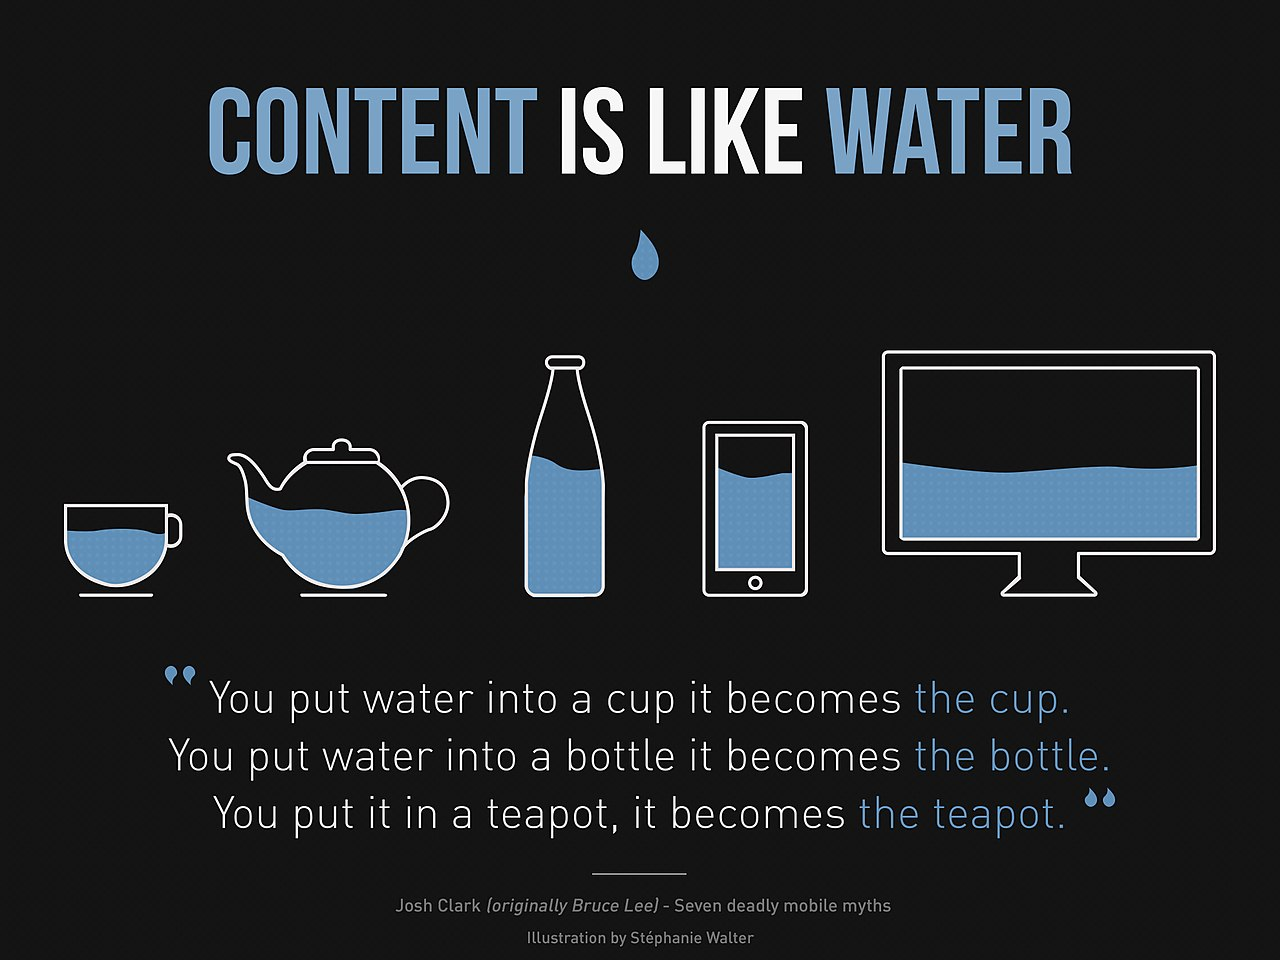
\includegraphics[width=\linewidth]{fluid.jpg}
	\end{figure}
\end{frame}

\begin{frame}{Jak nie robić?}	
	Zanim RWD zagościło na dobre w internecie, jednym ze sposobów na radzenie sobie z urządzeniami o mniejszej rozdzielczości było tworzenie specjalnych stron w "wersji mobilnej".
	
	Przykładem może być archaiczny \texttt{mobile.facebook.com}.
\end{frame}

\begin{frame}{Jak robić?}	
	Obecny trend to tworzenie jednej aplikacji frontendowej, która dynamicznie dopasowuje się do rozdzielczości urządzenia.
\end{frame}

\begin{frame}{Przykład: 1920px na szerokości}
	\begin{figure}[t]
		\centering
		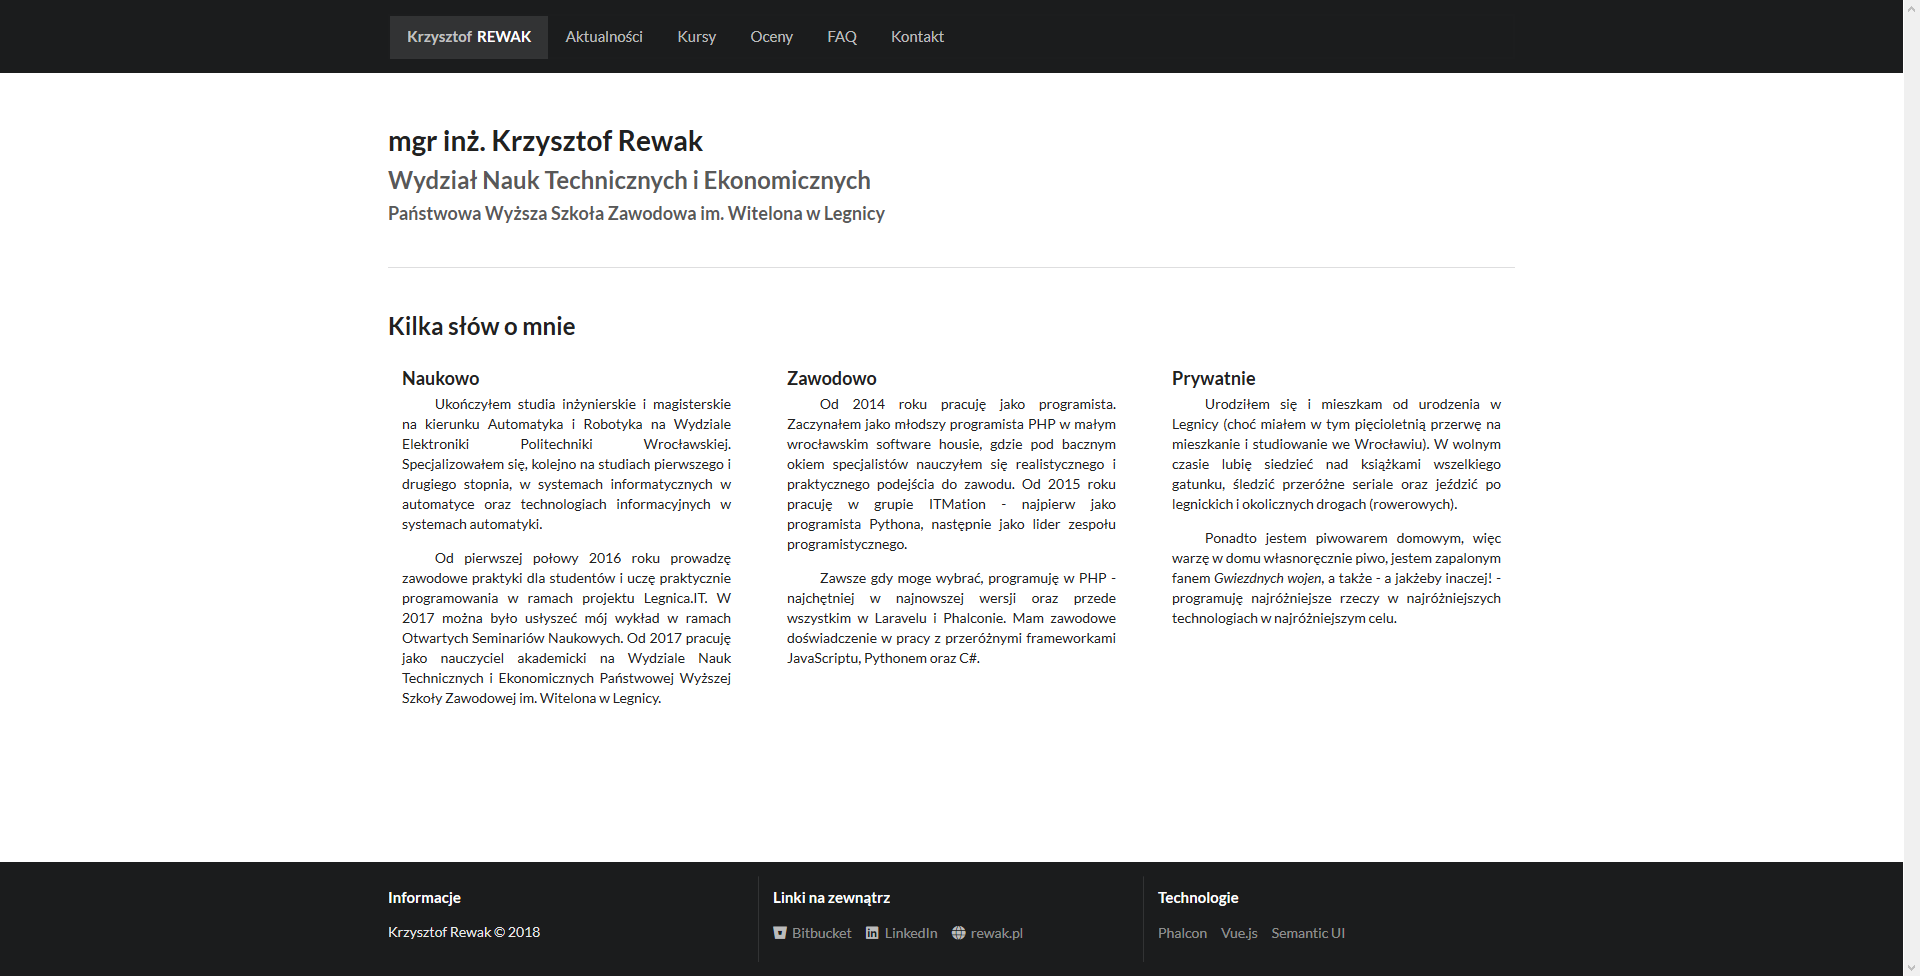
\includegraphics[width=\linewidth]{1920.png}
	\end{figure}
\end{frame}

\begin{frame}{Przykład: 1366px na szerokości}
	\begin{figure}[t]
		\centering
		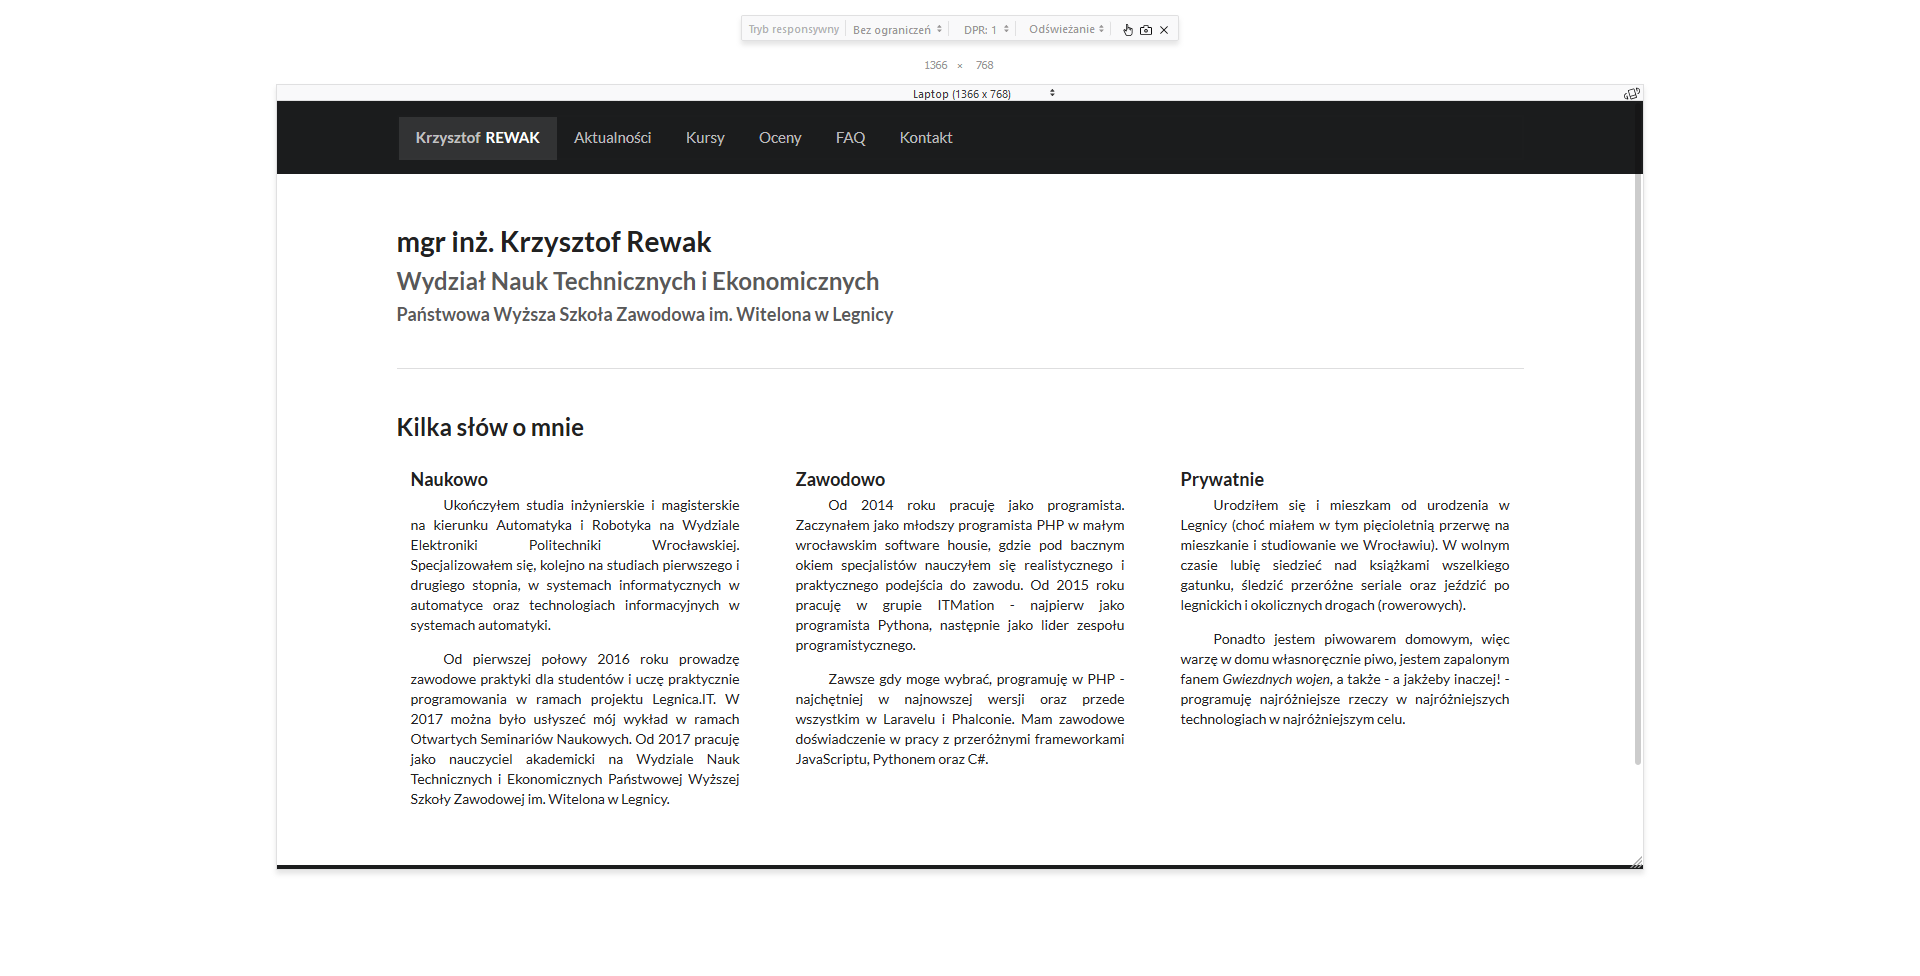
\includegraphics[width=\linewidth]{1366.png}
	\end{figure}
\end{frame}

\begin{frame}{Przykład: 1280px na szerokości}
	\begin{figure}[t]
		\centering
		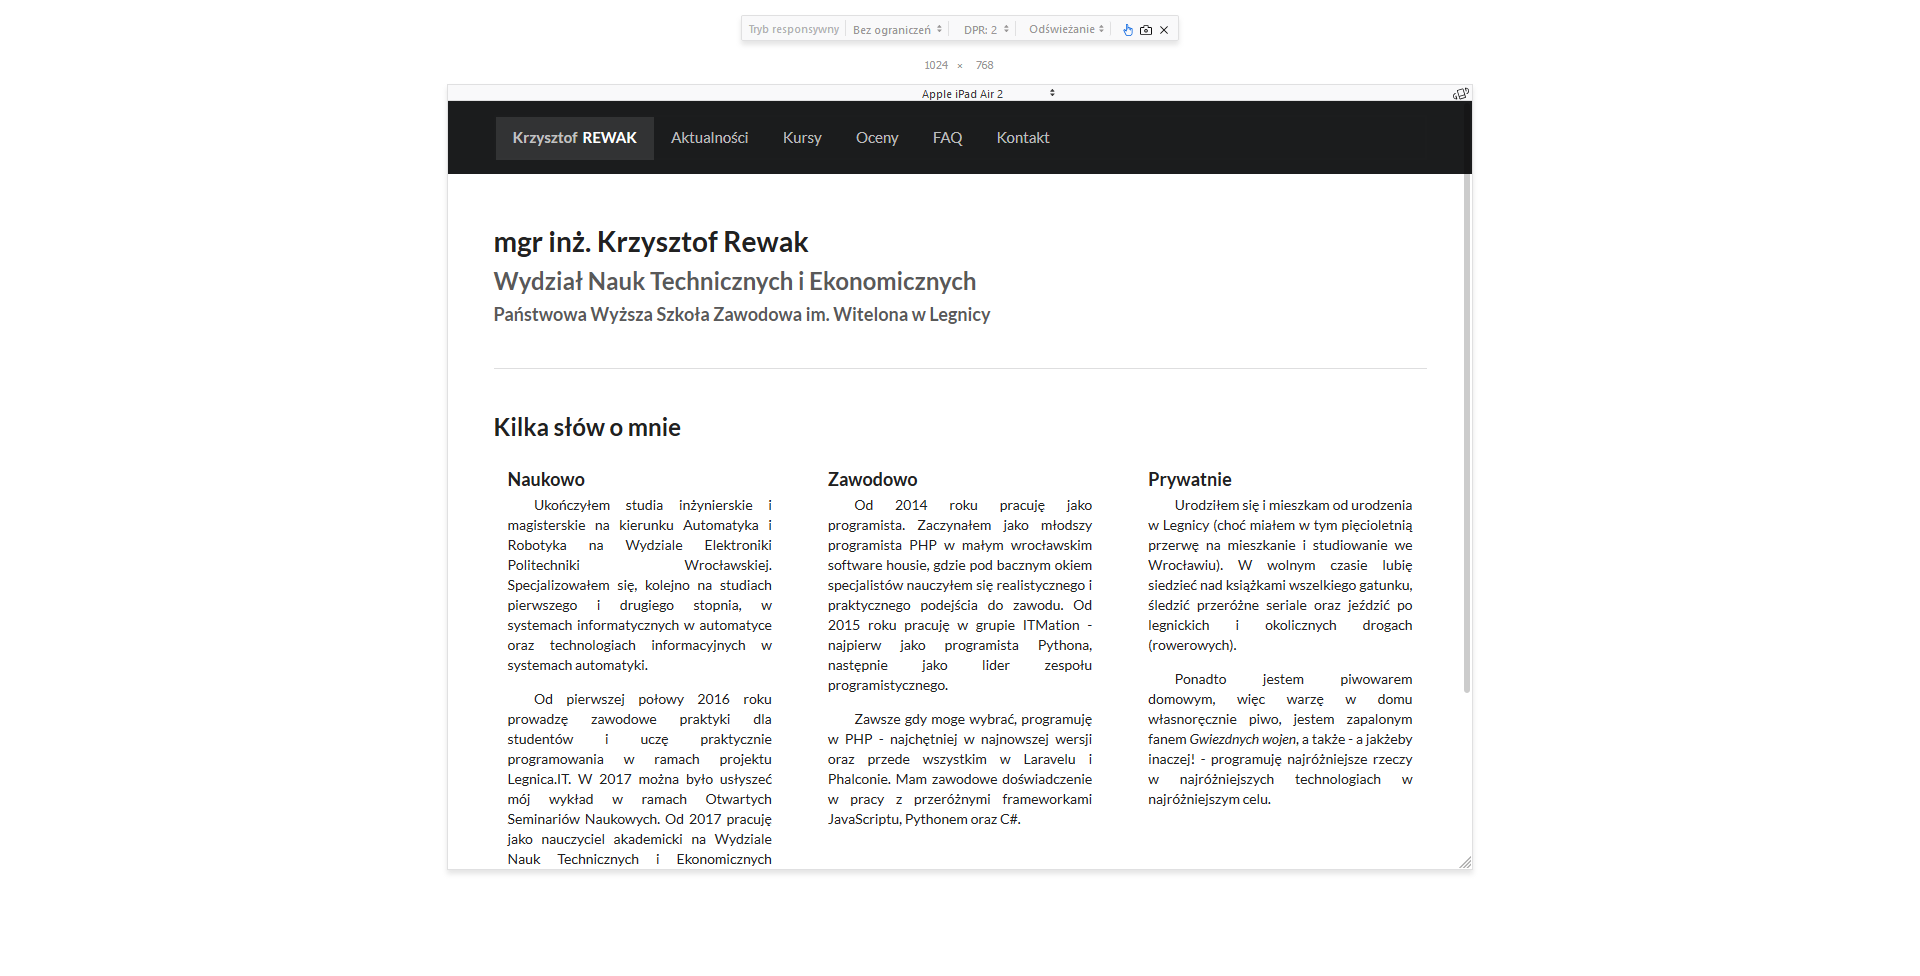
\includegraphics[width=\linewidth]{1024.png}
	\end{figure}
\end{frame}

\begin{frame}{Przykład: 667px na szerokości}
	\begin{figure}[t]
		\centering
		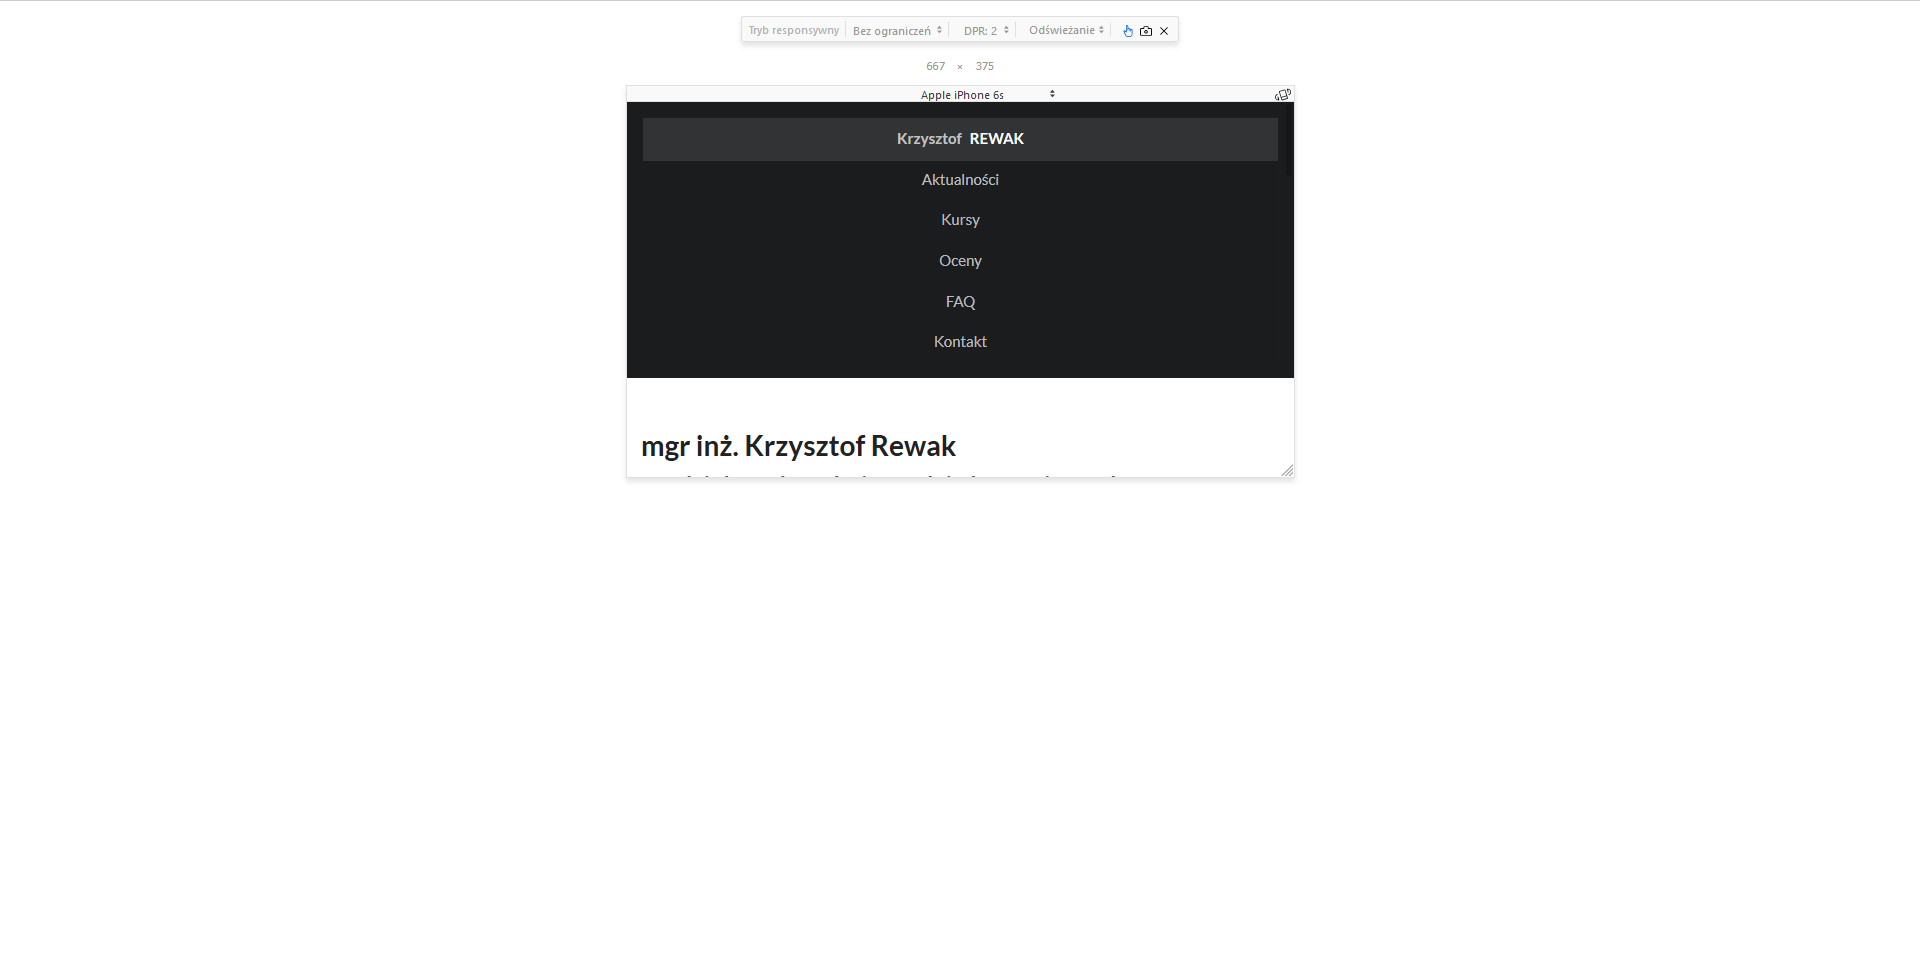
\includegraphics[width=\linewidth]{667.png}
	\end{figure}
\end{frame}

\begin{frame}{Przykład: 375px na szerokości}
	\begin{figure}[t]
		\centering
		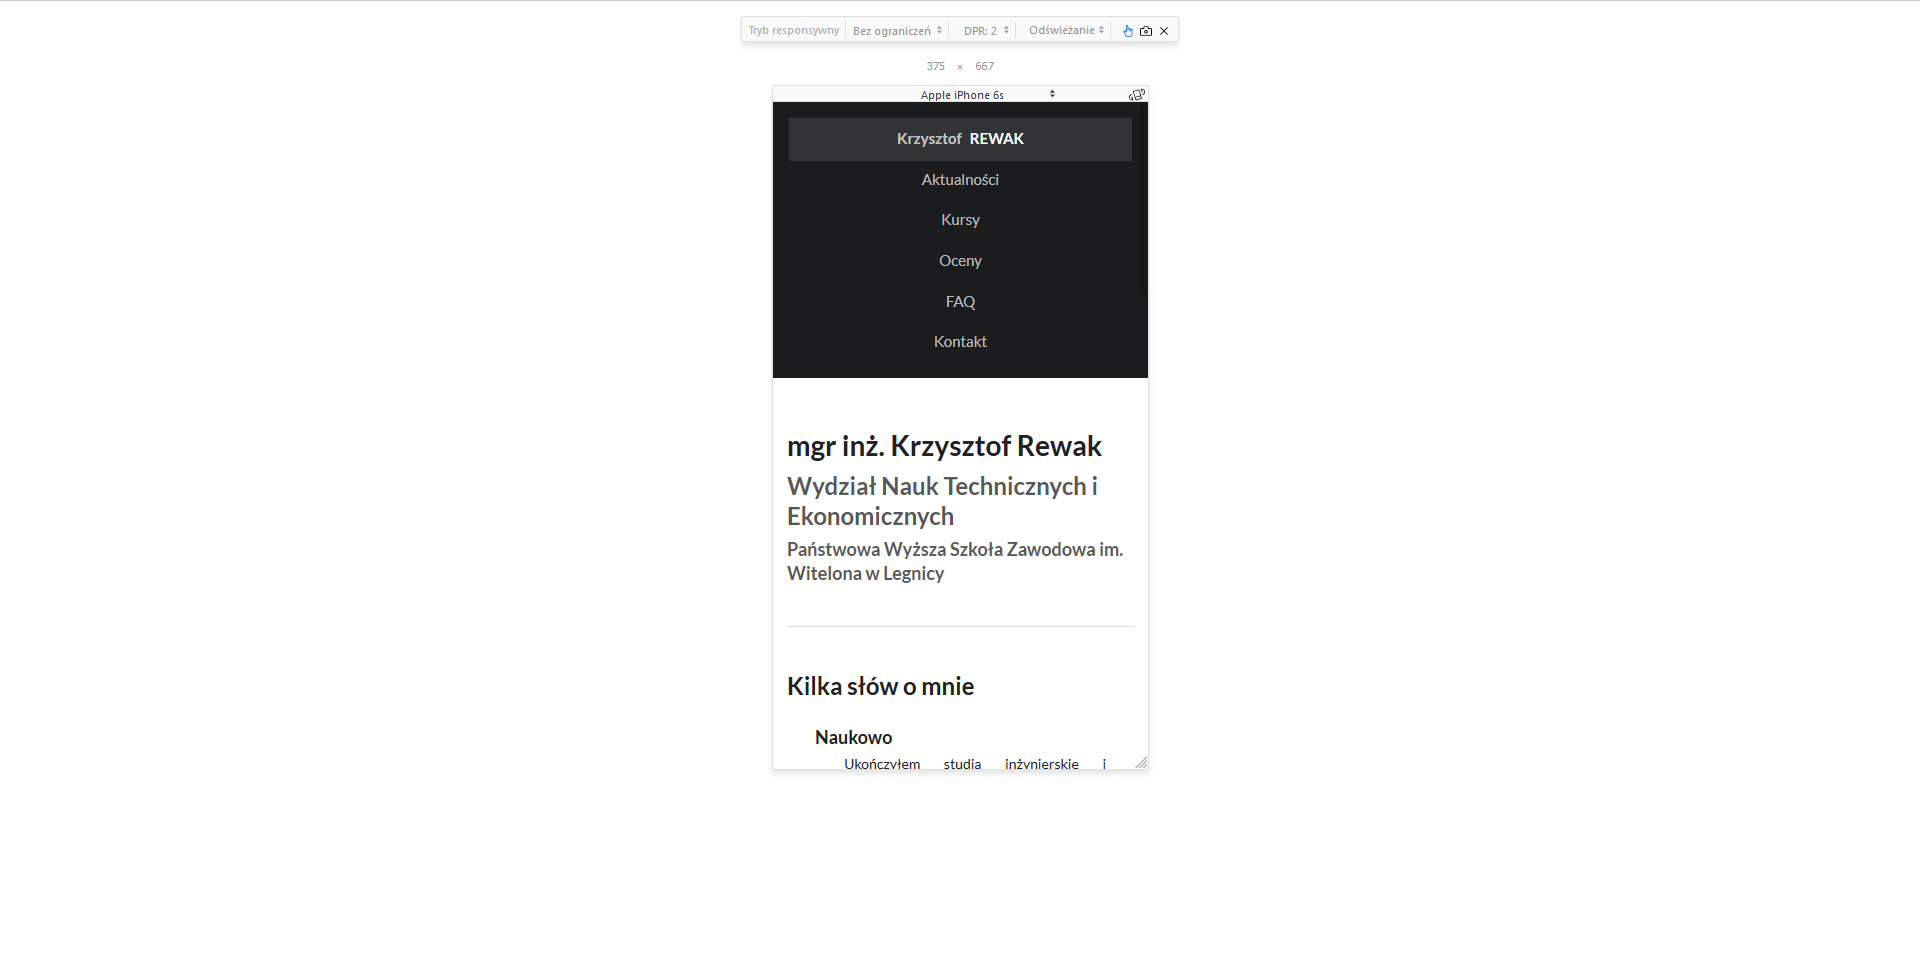
\includegraphics[width=\linewidth]{375.png}
	\end{figure}
\end{frame}

\begin{frame}[fragile]{Od strony kodu}
	\begin{lstlisting}
<div class="row">
    <div class="column">Content A</div>
    <div class="column">Content B</div>
    <div class="column">Content C</div>
</div>
	\end{lstlisting}
\end{frame}

\begin{frame}{Jak robić?}	
	Jak domyślnie będzie wyglądał przykład z poprzedniego slajdu?
	
	Będą to ułożone, jeden pod drugim, kontenery szerokości i wysokości dopasowanej do wstawionego w nich tekstu.
\end{frame}

\begin{frame}[fragile]{Od strony kodu}
	Co się stanie po dodaniu poniższych reguł CSS?
	\begin{lstlisting}
.row {
    
    width: 100%;

    .column {
        width: 33%;
        background: Red;
        display: inline-block;
    }

}
	\end{lstlisting}
\end{frame}

\begin{frame}[fragile]{Od strony kodu}
	Nic się nie stanie po dodaniu powyższych reguł. Należy je wpierw przetworzyć z Sass na CSS:
	\begin{lstlisting}
.row {
    width: 100%;
}

.row .column {
    width: 33%;
    background: Red;
    display: inline-block;
}
	\end{lstlisting}
\end{frame}

\begin{frame}{Co dalej?}	
	Wówczas każdy z kontenerów z tekstem zajmie 1/3 szerokości okna. Utworzy to system kolumn, w którym można wygodnie prezentować dane.
	
	Czasami jednak może źle się to wyświetlić na węższych ekranach.
\end{frame}

\begin{frame}[fragile]{\emph{Media queries}}
	Opcja \#1: stworzenie dwóch arkuszy dla różnych rozdzielczości ekranu:
	\begin{lstlisting}
<link
    rel="stylesheet"
    media="screen and (min-width: 900px)"
    href="widescreen.css">
    
<link
    rel="stylesheet"
    media="screen and (max-width: 600px)"
    href="smallscreen.css">
	\end{lstlisting}
\end{frame}

\begin{frame}[fragile]{\emph{Media queries}}
	Opcja \#2: wstawianie różnych reguł wewnątrz arkusza:
	\begin{lstlisting}
.row {
    
    width: 100%;

    .column {
        width: 33%;
        background: Red;
        display: inline-block;
    }
    
    @media screen and (max-width: 768px) {
        .column {
            width: 100%;
            display: block;
        }
    }

}
	\end{lstlisting}
\end{frame}

\begin{frame}{768px?}	
	Jak punkty brzegowe przyjąć przy tworzeniu responsywnego frontendu? Bootstrap wykorzystuje sensowny podział \emph{breakpointów}:
	\begin{itemize}
	\item do 576px dla urządzeń bardzo małych (np. telefonów w pozycji pionowej)
	\item do 768px dla urządzeń małych (np. telefonów w pozycji poziomej)
	\item do 992px dla urządzeń średnich (np. tabletów)
	\item do 1200px dla urządzeń dużych (głównie laptopów)
	\item powyżej 1200px dla urządzeń bardzo dużych
	\end{itemize}
\end{frame}

\begin{frame}{Jakich rozdzielczości się używa?}
	\begin{figure}[t]
		\centering
		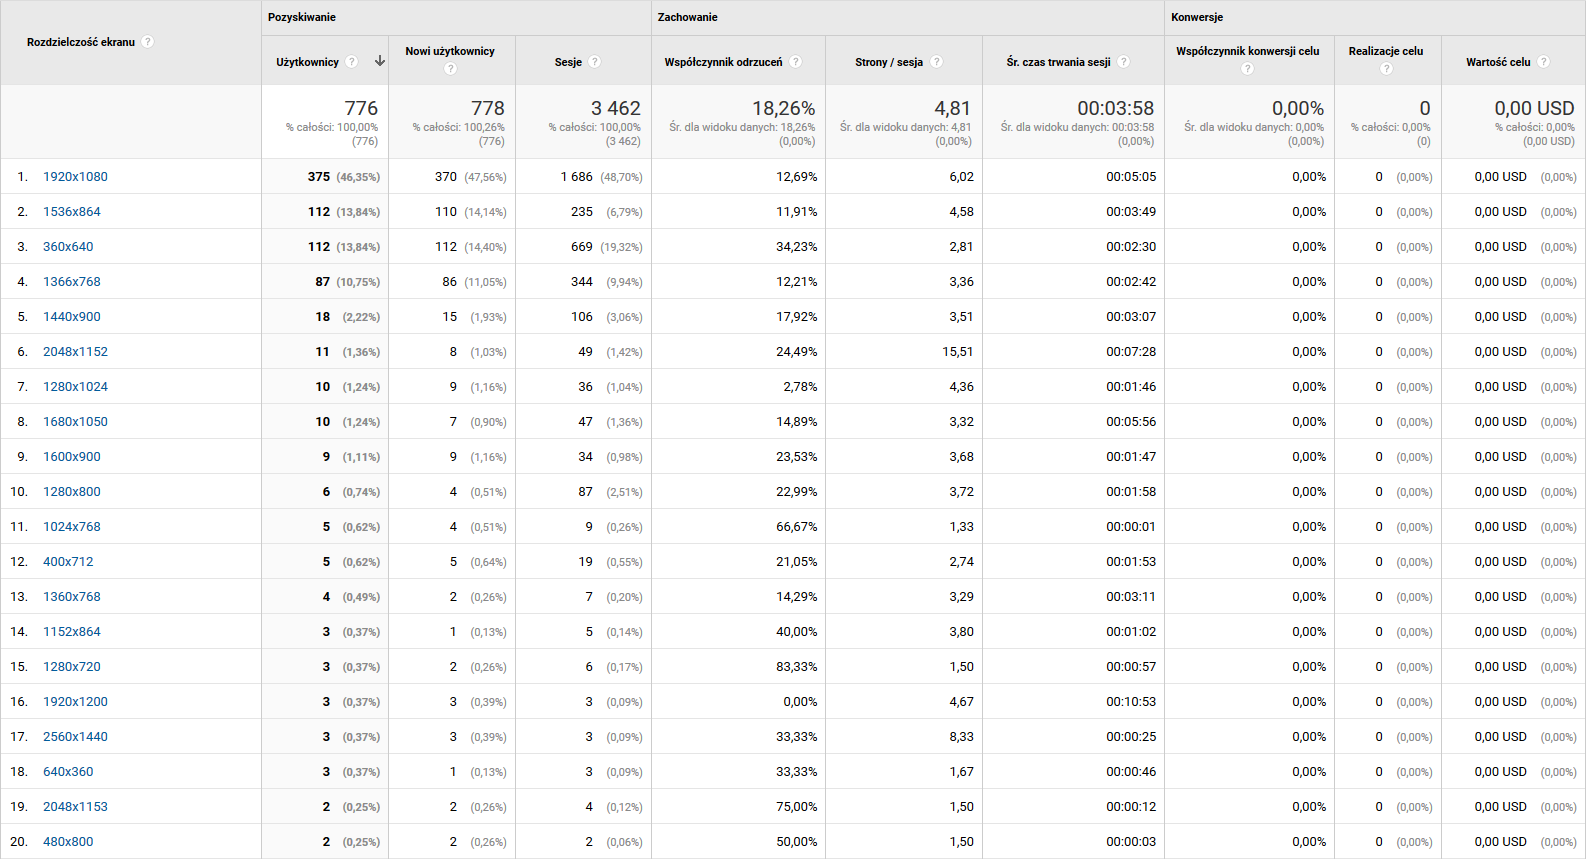
\includegraphics[width=\linewidth]{ga.png}
	\end{figure}
\end{frame}

\begin{frame}[fragile]{Bootstrap to obecnie standard}
	Poniższy kod utworzy wiersz z trzema kolumnami równej szerokości, ale na ekranach o rozdzielczości mniejszej niż 576px kolumny ustawią się jedna nad drugą.

	\begin{lstlisting}
<div class="container">
  <div class="row">
    <div class="col-sm">
      One of three columns
    </div>
    <div class="col-sm">
      One of three columns
    </div>
    <div class="col-sm">
      One of three columns
    </div>
  </div>
</div>
	\end{lstlisting}
\end{frame}

\begin{frame}{Zastosowania}	
	Do czego można wykorzystać RWD?
	\begin{itemize}
	\item ukrycie paska nawigacyjnego pod tzw. \emph{hamburger menu}
	\item przemieszczenie bocznych pasków (najczęściej lewy nad zawartość, prawy pod)
	\item zmiana umieszczenia przycisków/tagów (normalnie jeden obok drugiego, na małych ekranach - pod sobą, ale wypełniające całą szerokość ekranu)
	\item marginesy wewnętrzne i zewnętrzne różnie wyglądają na różnej wielkości ekranach
	\item itd. itp.
	\end{itemize}
\end{frame}

\section{SPA}

\begin{frame}{SPA}	
	\textbf{SPA} (od ang. \emph{single-page application}) to podejście w projektowaniu aplikacji internetowych polegające na tworzeniu frontendu, który nie wymaga przeładowania strony.
\end{frame}

\begin{frame}{SPA}	
	Wykorzystywane są w tym celu asynchroniczne odpytywania serwera, czyli AJAX.
\end{frame}

\begin{frame}{SPA}
	\begin{figure}[t]
		\centering
		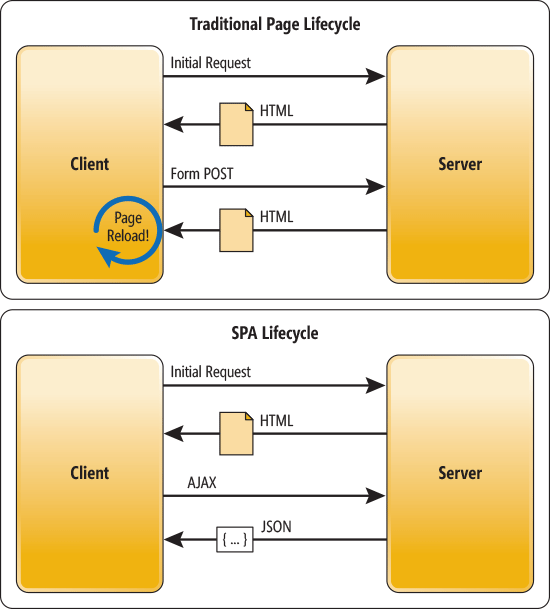
\includegraphics[width=.65\linewidth]{spa.png}
	\end{figure}
\end{frame}

\begin{frame}{Jak wygląda taka aplikacja?}	
	Dobrze skonstruowana SPA powinna składać się z jednego pliku \texttt{index.html} oraz plików pomocnicznych (przede wszystkim JavaScript, CSS, grafiki, fonty).
	
	Pliki pomocnicze można umieścić na CDN-ie.
\end{frame}

\begin{frame}{Jak wygląda taka aplikacja?}	
	\begin{figure}[t]
		\centering
		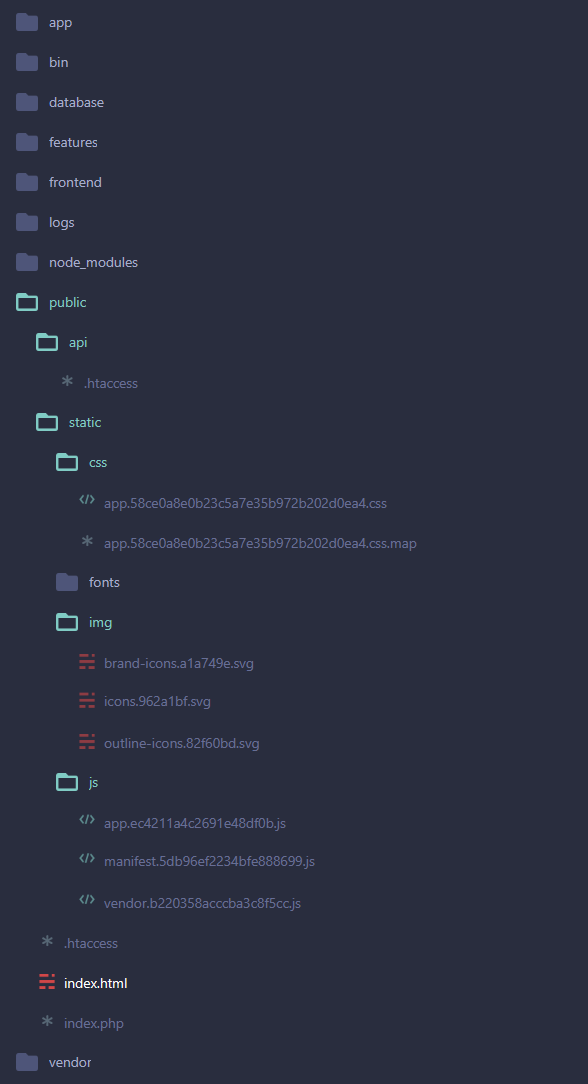
\includegraphics[width=.4\linewidth]{folders.png}
	\end{figure}
\end{frame}

\begin{frame}{Jak wygląda taka aplikacja?}	
	Wszelkie \emph{dynamiczne }informacje powinny zostać pobrane z API wystawionego na backendzie. Backend ten może funkcjonować zarówno na tej samej instancji serwera co frontend, jak i na całkiem innej maszynie z innym adresem.
\end{frame}

\begin{frame}{Pułapki}	
	Domyślnie SPA mogą mieć problem z przekierowaniem użytkownika na wybraną stronę. Rozwiązaniem może być wykorzystanie routera będącego częścią współczesnych frameworków frontendowych.
\end{frame}

\begin{frame}{Router}	
	W kodzie JavaScriptowym umieszcza się listę ścieżek i akcji jakie mają zostać zrealizowane po wejściu na ścieżkę. Odpowiednie reguły w ustawieniach serwera HTTP przekierują cały ruch na plik \texttt{index.html} z załączonym routerem, który zajmie się wywołaniem odpowiedniej akcji.
\end{frame}

\begin{frame}{Router}
	\begin{figure}[t]
		\centering
		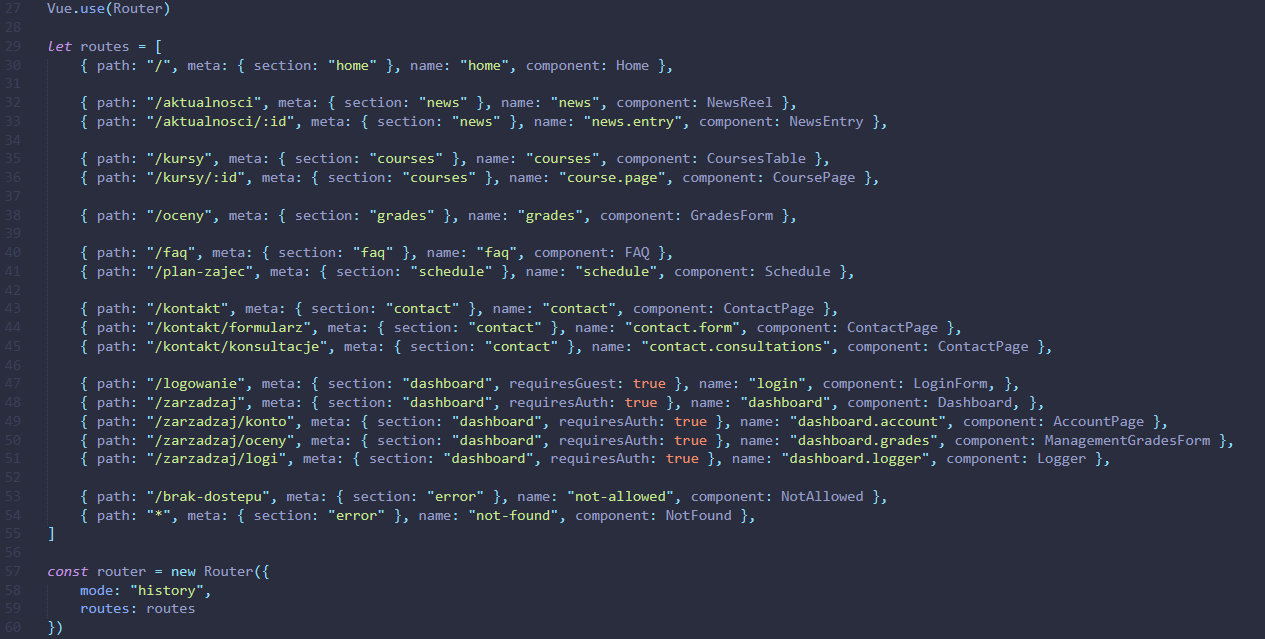
\includegraphics[width=\linewidth]{router.png}
	\end{figure}
\end{frame}

\begin{frame}{Zastosowania}	
	SPA mają różnorodne zastosowania:
	\begin{itemize}
	\item małe witryny firm,
	\item panele adminstracyjne systemów zarządzania treścią,
	\item panele administracyjne systemów typu CRM lub ERP,
	\item portale społecznościowe...
	\end{itemize}
	
	Czyli praktycznie wszystko, co można obejrzeć w internecie.
\end{frame}

\begin{frame}{Plusy i minusy}
	Plusy:
	\begin{itemize}
	\item wygodne i \emph{efektowne} dla użytkownika,
	\item pełne odseparowanie back- i frontendu,
	\item zmniejszenie czasu wczytywania strony.
	\end{itemize}
\end{frame}

\begin{frame}{Plusy i minusy}
	Minusy:
	\begin{itemize}
	\item trzeba poznać nową (i często niestabilną) technologię,
	\item trzeba konfigurować drugie (frontendowe) środowisko,
	\item nie wszystkie przeglądarki będą działały tak samo.
	\end{itemize}
\end{frame}

\section{SEO}

\begin{frame}{SEO}
	\textbf{SEO} (od ang. \emph{search engine optimization}) to podejście w projektowaniu aplikacji internetowych polegające na zwiększaniu przewidywanej pozycji witryny w wynikach wyszukiwarek internetowych.
	
	Polska często spotykana nazwa to \textbf{pozycjonowanie}.
\end{frame}

\begin{frame}{SEO}
	Jakie są narzędzia SEO?
	
	Trudno odpowiedzieć w prosty i jednoznaczny sposób. Rynek wyszukiwarek zmienia się dynamicznie i ciężko sprecyzować sensowny sposób na SEO.
\end{frame}

\begin{frame}{\texttt{<meta>}}
	Podstawowym narzędziem wstępnej optymalizacji pod wyszukiwarki jest uzupełnienie tagów \texttt{<meta>} w nagłówku strony internetowej.
\end{frame}

\begin{frame}{\texttt{<meta>}}
	\begin{figure}[t]
		\centering
		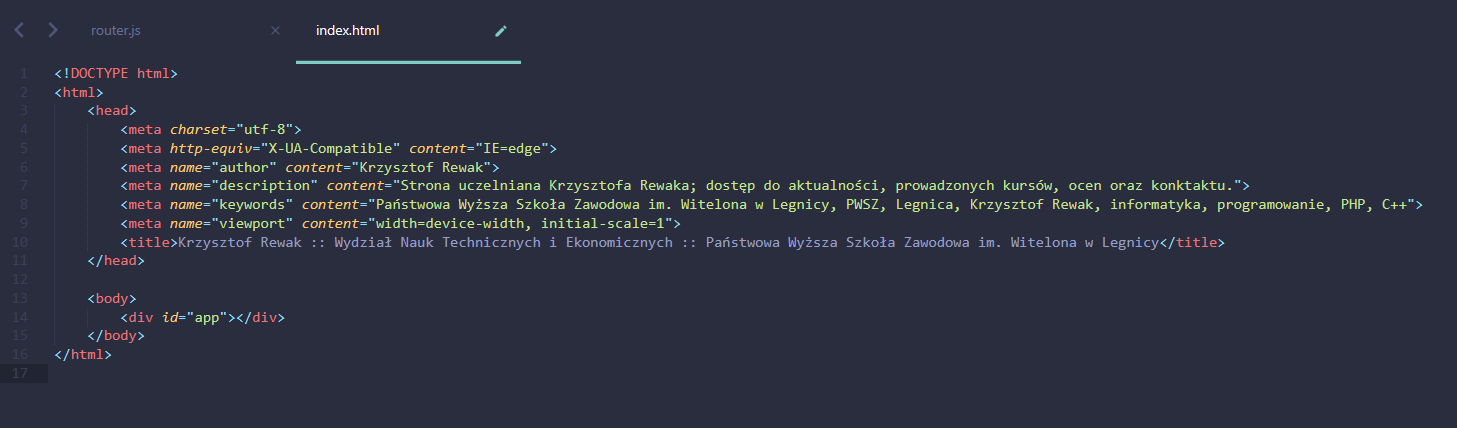
\includegraphics[width=\linewidth]{meta.png}
	\end{figure}
\end{frame}

\begin{frame}{\texttt{<meta>}}
	Stety-niestety nadużycia tejże formy spowodowały, że boty Google i innych wyszukiwarek skanują obecnie całe strony w poszukiwaniu \emph{organicznych} słów kluczowych.
\end{frame}

\begin{frame}{Jak nie ogarniać SEO?}
	Jak popsuć swój wynik w Google?
	\begin{itemize}
	\item zamieszczać nieprawdziwe dane, słowa kluczowe,
	\item zamieszczać zbyt wiele słów kluczowych,
	\item ukrywać elementy przed użytkownikiem,
	\item być linkowanym ze stron ze słabym wskaźnikiem SEO,
	\item budować zły kod.
	\end{itemize}
\end{frame}

\begin{frame}{Jak ogarnąć SEO?}
	Jak poprawić swój wynik w Google?
	\begin{itemize}
	\item umieścić mapę strony;
	\item sensownie używać HTML;
	\item oczyścić znaczniki HTML;
	\item uzupełnić tagi HTML;
	\item \emph{pretty URLs} i sensowne zawartości linków;
	\item stworzyć responsywny layout,
	\item i wiele, wiele innych.
	\end{itemize}
\end{frame}

\begin{frame}{Google PageSpeed Tools}
	\begin{figure}[t]
		\centering
		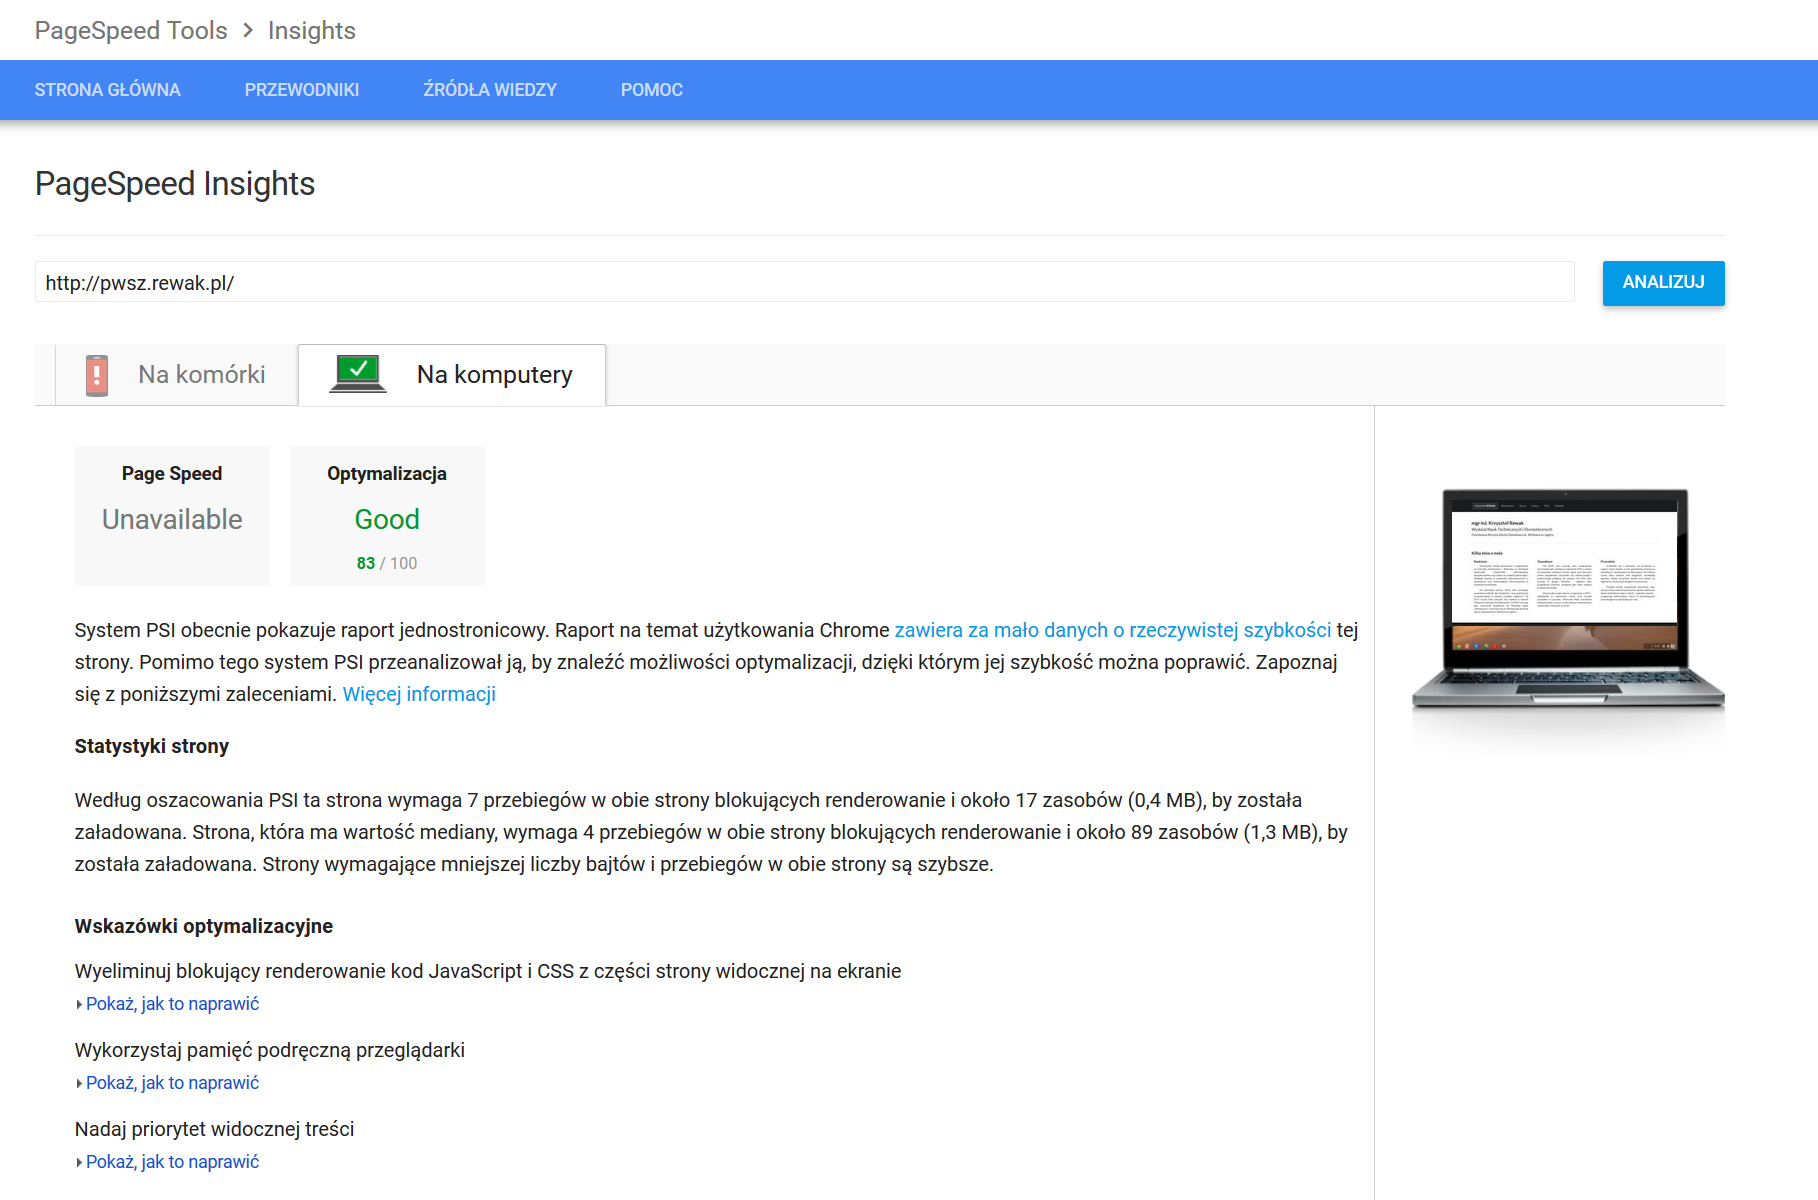
\includegraphics[width=\linewidth]{pagespeed1.png}
	\end{figure}
\end{frame}

\begin{frame}{Google PageSpeed Tools}
	\begin{figure}[t]
		\centering
		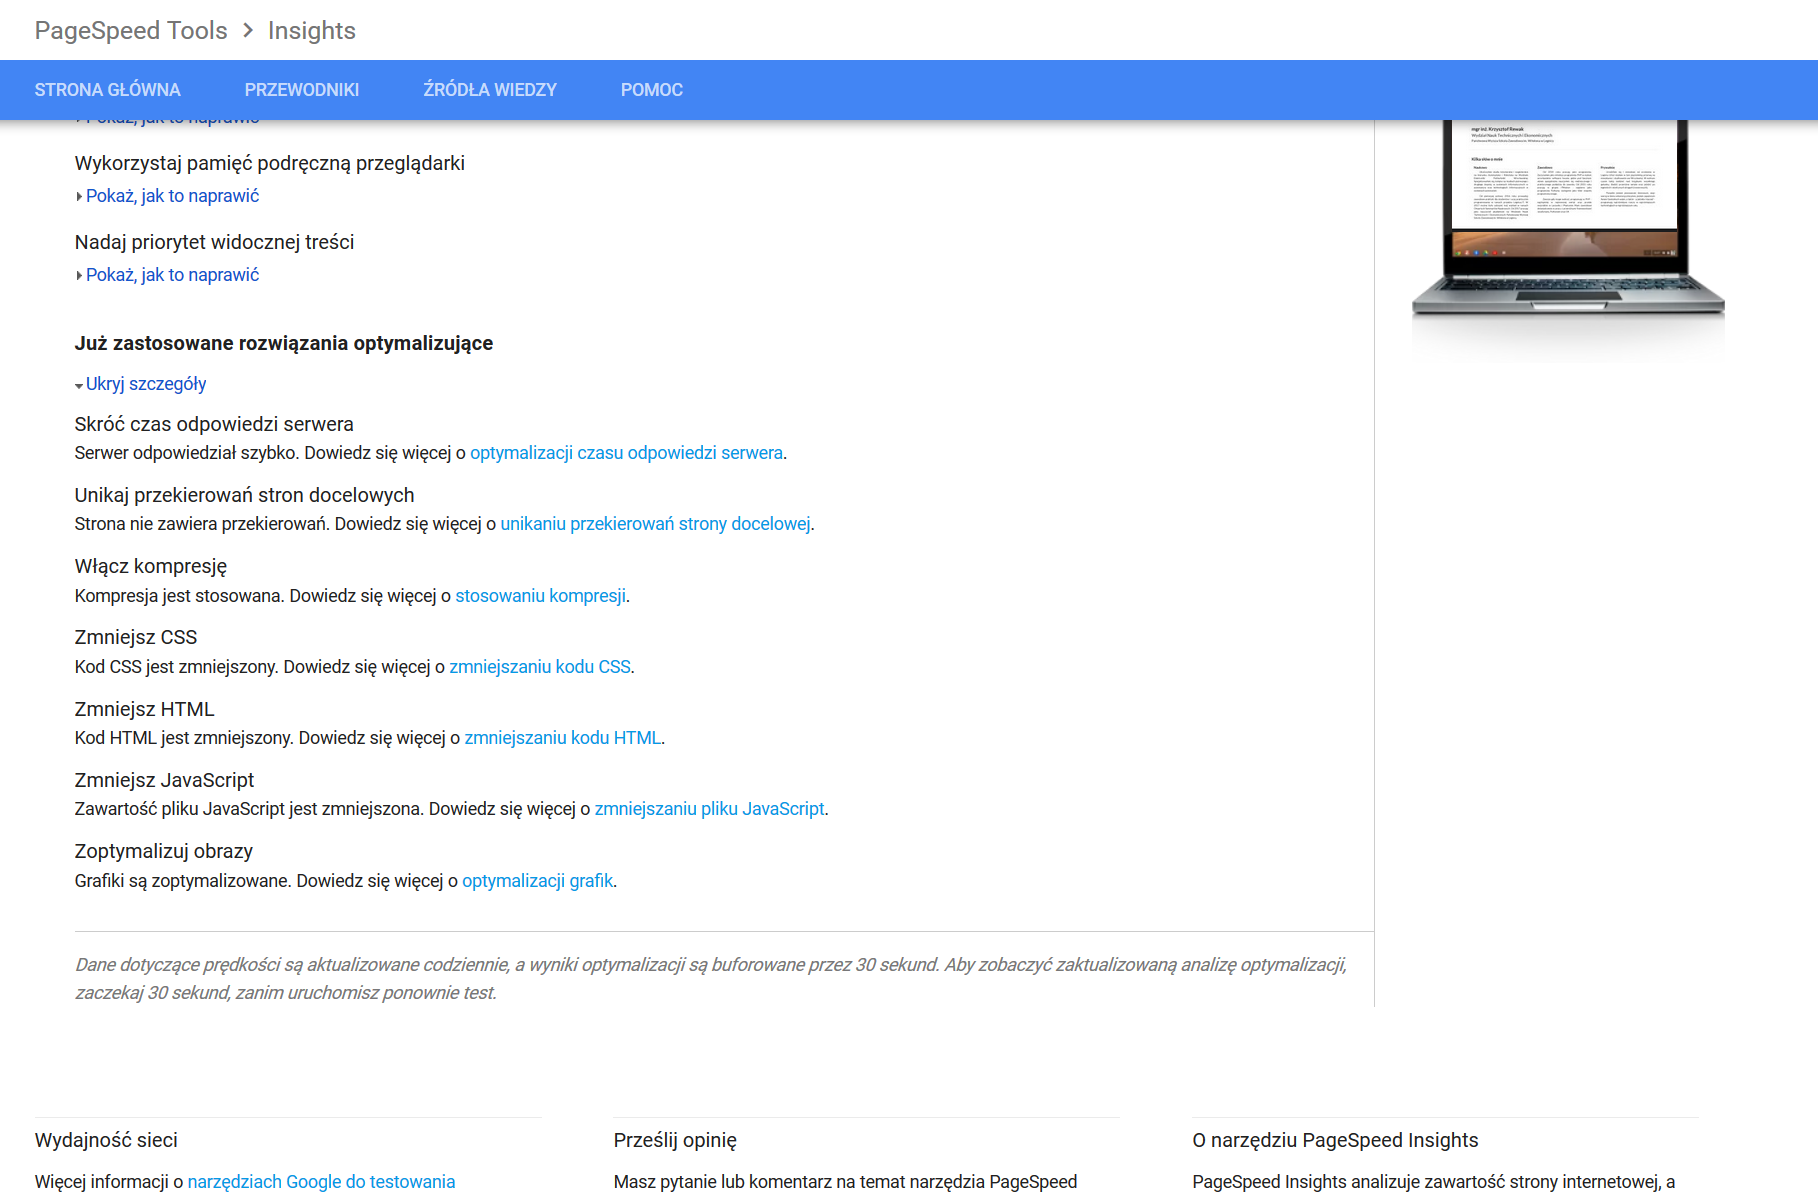
\includegraphics[width=\linewidth]{pagespeed2.png}
	\end{figure}
\end{frame}

\section{Podsumowanie}

\begin{frame}{Bibliografia i ciekawe źródła}
  
	\begin{thebibliography}{9}
		
		\bibitem{medias}
		\url{https://www.w3schools.com/cssref/css3_pr_mediaquery.asp}
		
		\bibitem{grid}
		\url{https://getbootstrap.com/docs/4.1/layout/grid/}
		
		\bibitem{spa}
		\url{https://msdn.microsoft.com/en-us/magazine/dn463786.aspx}
		
		\bibitem{pagespeed}
		\url{https://developers.google.com/speed/pagespeed/insights/}
		
	\end{thebibliography}

\end{frame}

\appendix

\begin{frame}[standout]
	Pytania?
\end{frame}

\begin{frame}{}

	Kod prezentacji dostępny jest w repozytorium git pod adresem \texttt{https://bitbucket.org/krewak/pwsz-ppsi} \\ \ \\

	\begin{figure}
		\centering
		\href{https://bitbucket.org/krewak/pwsz-ppsi}{
			
\includegraphics[width=.15\textwidth]{../_template/bitbucket.png}
		}
	\end{figure}
	
	Wszystkie informacje dot. kursu dostępne są pod adresem \texttt{http://pwsz.rewak.pl/kursy/4} \\ \ \\

	\begin{figure}
		\centering
		\href{http://pwsz.rewak.pl/kursy/3}{
			
\includegraphics[width=.15\textwidth]{../_template/rewak.png}
		}
	\end{figure}

\end{frame}

\end{document}
